\chapter{High-Throughput Imaging using Coded Illumination}

High-throughput wide-field microscopy enables the collection of large amounts of image data at high-speed, using optimized hardware and computational techniques to push system throughput beyond conventional limits. These systems play a critical role in many fields, including drug-discovery~\cite{Perlman1194, brodin2011high, bickle2010beautiful}, functional protein analysis~\cite{Liebel:03, huh2003global} and neuropathology~\cite{peiffer1979alcohol, remmelinck2000could, alegro2017automating}, enabling the rapid acquisition of large volumes of data. In wide-field microscopes, the choice of objective lens imposes a trade-off between both the resolution and field of view (FOV) of the system. Addressing this trade-off has been the subject of a large number of computational imaging techniques~\cite{Zheng2013, betzig2006imaging, Rust:06, gustafsson2000surpassing, rodenburg2004phase, Tian2014}, which have, through various mechanisms, demonstrated the ability to enhance the resolution of an imaging system beyond the wide-field diffraction limit while maintaining the same FOV. Similarly, system throughput may also be enhanced by increasing the FOV directly through mechanical scanning and image-stitching while maintaining the resolution of the imaging optics. This direct approach has been widely employed for commercial slide-scanning systems~\cite{zeissSlideScan}, which, when coupled with state of the art analysis tools such as CellProfiler~\cite{Carpenter2006}, have enabled statistical analysis of the cellular micro-environment at larger scales than ever before.

Despite their wide adoption for a large variety of imaging tasks, the performance of slide-scanning systems is often limited by the mechanical parameters of the motion stage rather than the camera, leading to lower information throughput than comparable computational imaging systems which employ coded illumination. These mechanical motions can lead to long acquisition times, especially when imaging very large samples such as coronal sections of the human brain~\cite{Grinberg2007} at cellular resolution. Conversely, a Fourier-domain super-resolution technique such as Fourier ptychography only requires electronic scanning of LED illumination, so is more likely to be limited by photon counts or camera readout, since the time to change LED patterns is on the order of microseconds. However, most super-resolution methods have a fixed FOV, requiring additional mechanical scanning to capture extended samples.

Conventional slide-scanning microscopes employ one of two imaging strategies. The first, commonly referred to as "stop-and-stare" involves moving the sample to each scan position serially, halting the stage motion before each exposure and resuming motion only after the exposure has finished. While this method produces high-quality images due to long exposures, it is slow due to the time required to stop and start motion between exposures. A second approach, often referred to as "strobed illumination", involves illuminating the sample with a very short, bright pulse as it moves continuously, such that the motion blur which would otherwise be introduced by an extended pulse is avoided. While fast, acquisitions performed under strobed illumination will generally produce images with much lower signal-to-noise ratio (SNR) than a comparable stop-and-stare acquisition due to short pulse times (often on the order of micro-seconds). The choice between these two acquisition strategies requires user to trade SNR for acquisition rate, often in ways which make large-scale imagery impractical due to extremely long acquisition times.

In the following sections, we will describe a technique for improving the speed of real-space scanning techniques by multiplexing using motion deblurring and coded illumination. Multiplexing was previous applied to Fourier ptychography~\cite{Tian2014} by illuminating LEDs from different angles during each frame, reducing acquisition times and increasing measurement SNR. This work presents a similar technique, where LED intensities are coded in time as the sample is moved continuously, and the resulting image is deconvolved using the known illumination sequence to recover the static image. Further, we show situations where our method is sub-optimal compared to the current state-of-the-art techniques in both theory and experiment\footnote{This work was performed in collaboration with Sarah Dean and Benjamin Recht (ADEPT Lab, EECS, UC Berkeley).}.

\section{Quantifying Throughput in Microscopy Systems}
The information throughput of an imaging system can be quantified by the space-bandwidth product (SBP), which is the dimensionless product of the spatial coverage (FOV) and Fourier coverage (resolution) of a system~\cite{Lohmann1996space}, as well as the space-bandwidth rate (SBR), which is SBP per unit time. Improving the SBP and SBR has been the subject of several seminal works in the field of computational imaging, including structured illumination~\cite{gustafsson2000surpassing}, localization microscopy~\cite{Rust:06, betzig2006imaging}, and both conventional~\cite{rodenburg2004phase} and Fourier~\cite{Zheng2013,tian2015computational,Tian2014} ptychography. While these methods are diverse in their approaches and application spaces, they share a common theme of acquiring multiple wide-field measurements under diverse imaging conditions to improve the throughput of an imaging system.

Evaluating the space-bandwidth product in conventional imaging systems involves comparing the minimum resolution enabled by the optical system with the aberration-free FOV shape. If a camera is perfectly matched to the resolution and FOV supported by the imaging optics, this is equivalent to counting the number of pixels on the camera. Practically, this is rarely the case, since camera pixels are rectangular and the optical point-spread function (PSF) is generally circular (owing to the circular shape of most camera apertures). The nominal optical FOV in a microscope is normally set based on the quality of the optical designs used in the objective lens; calculating this is beyond the scope of this work (although Chapter~\ref{ch:selfcal}, Section~\ref{sec:selfcal:dpc} illustrates the graduation degradation of resolution across the FOV). Practically, the camera is what defines the FOV, as most system designers aim to image within the center of the FOV which generally has little aberration. The minimum resolution, however, is readily calculated from the system numerical aperture $NA$ using the Rayleigh criterion~\cite{rayleigh1896xv}:
\begin{equation}\label{eq:highthtoughput_rayleigh}
    \Delta x = \frac{1.22 \lambda}{NA}
\end{equation}

\noindent where $\lambda$ is the illumination wavelength. This resolution limit defines the maximum spatial frequency in the optical system, which is related to the numerical aperture of the camera by the simple relation:
\begin{equation}
    k_{max} = \frac{NA}{\lambda}
\end{equation}

The camera sampling must be chosen such that this maximum spatial frequency is sampled as the Nyquist rate, which is $2k_{max}$. Practically, this is accomplished by introducing magnification to the optical system to shrink the pixel shape to match the required spatial frequency. Mathematically, the goal is to determine a magnification factor $M$ which satisfies the following bound, given a camera pixel size $\Delta$:

\begin{equation}
    \frac{\Delta}{M} \leq \frac{1}{2k_{max}}
\end{equation}

For color imaging system, note that the factor $\Delta$ must be doubled, since measurements at each color channel occur at twice the distance between each measurement.

Assuming these criterion are met, the total bandwidth of the system is set by the system resolution (Eq.~\ref{eq:highthtoughput_rayleigh}) and the sensor shape scaled by the magnification. The Wigner Distribution Function (WDF)~\cite{BASTIAANS197826}) provides an intuitive geometric description of the aspect ratio of the system coverage in the spatial and spectral dimensions as a function of the prescribed resolution and FOV as set by the system magnification. For example, the SBP of a 10$\times$ / 0.25NA and a 40$\times$ / 1.0NA objective may be the same, but the former will allocate more throughput to resolution than FOV, while the latter will provide a wide FOV at lower resolution. This well-known trade-off is illustrated in Figure~\ref{fig:highthroughput_sbp}.

\begin{figure*}
  \centering
    \includegraphics[width=\textwidth]{figures/fig_highthroughput_sbp.png}
  \caption{\label{fig:highthroughput_sbp} Illustration of ideal space-bandwidth product allocation for various common objective lenses as plotted in the WDF. While the area of each rectangle remains constant, the aspect ratio illustrates the allocation of bandwidth between high-resolution and a wide FOV.}
\end{figure*}

The illustration in Fig.~\ref{fig:highthroughput_sbp} reveals the regions which are most amenable to scanning for common objective types. For example, when using an objective with a high magnification and NA, it would be more optimal to scan a sample in the real domain, since each measurement will already have significant spectral coverage (resolution). Conversely, low-magnification optics are more amenable to scanning in the frequency domain to build resolution, since these systems already have a very large FOV. This intuition explains the practical benefits of performing Fourier ptychography using a low-magnification objective~\cite{Zheng2013}, since scanning is performed in the frequency domain - there would be little practical benefit to performing Fourier ptychography using a high-magnification objective and the maximum illumination NA would be roughly the same as the imaging NA (making any resolution improvement marginal compared to brightfield or DPC phase imaging).

On the other hand, mechanical scanning provides a means for augmenting the SBP in real-space, making it amenable for high-magnification imaging systems. A basic example of this technique is slide-scanning systems, which move a sample while serially capturing images between each movement. A second example is conventional ptychography~\cite{rodenburg2004phase}, which probes a sample in real-space while imaging the diffracted field in the Fourier domain (usually using propagation onto a detector array). The choice of which scanning method to use is a general question and is beyond the scope of this work, but would certainly depend on the relative acquisition bottlenecks present in each system, and would be best compared using the SBR. Figure~\ref{fig:highthroughput_scanning} illustrates these two scanning techniques.

\begin{figure*}
  \centering
    \includegraphics[width=0.75\textwidth]{figures/fig_highthroughput_scanning.png}
  \caption{\label{fig:highthroughput_scanning} Comparison of spectral and spatial scanning techniques in high-throughput systems.}
\end{figure*}

A final parameter of interest is the signal-to-noise ratio (SNR) of the recovered images. In imaging, SNR is generally defined as ratio of the mean signal to the standard deviation of the background (As described in Eq.~\ref{eq:intro_snr}). The absolute SNR requirements vary based on applications; generally speaking, a $SNR > 10$ is considered a threshold where images have good SNR, although images below this threshold are also useful for many applications. The SNR is inherently tied to space-bandwidth rate because SNR will always increase for larger exposure times, which would conversely lead to a lower SBR due to longer dwell times for each measurement. Therefore, it is important to consider a minimum SNR as an additional constraint on the speed of the optical system. Practically, this trade-off is most noticeable under strobed illumination, where a dim illumination source and short exposure time can cause low measurement SNR. Decreasing sample velocity will increase SNR, but at the cost of a slower overall acquisition. The remaining sections of this paper present a method for increasing the SNR of measurements, which could also be interpreted as increasing the maximum SBR to maintain a necessary minimum signal-to-noise ratio.

\begin{figure*}
  \centering
    \includegraphics[width=0.8\textwidth]{figures/fig_highthroughput_system.pdf}
  \caption{\label{fig:system}High throughput imaging system with coded illumination. A.) Our system consists of an inverted optical fluorescence microscope with a 2-axis motion stage, illuminated using a programmable LED illumination source. In our proposed method, the sample is illuminated with many discrete pulses while being scanned at constant velocity. B.) Comparison between conventional high-throughput imaging techniques (stop-and-stare, strobed illumination) and our proposed coded illumination technique. Coded illumination provides a trade-off between SNR and acquisition speed, particularly for low-light situations such as fluorescence imaging. C.) Image of our system, which is a Nikon TE300 microscope configured with a Prior motion stage and LED illuminator.}

\end{figure*}

\section{High-Throughput Microscopy with Motion Deblurring}
In this section, we propose a novel computational imaging technique which employs a coded-illumination acquisition and deconvolution to meet the demands of high-throughput applications which require a minimum SNR. Our method involves illumination the sample with multiple pulses during each acquisition in order to improve the SNR compared to strobed illumination, while maintaining a high acquisition rate. With knowledge of this pulse sequence and motion trajectory, the blurred image can be used to perform a reconstruction of the static image, with higher SNR than a comparable strobed acquisition. Our method employs a motion-multiplexing technique to enhance the measurement SNR of our system by illumination with a sequence of short, bright pulses every frame. The captured images contain motion-blur artifacts, which must be removed computationally through a motion deblurring algorithm~\cite{raskar2006coded}. The overall gain in SNR is proportional to the number of pulses as well as the conditioning of the motion deblurring process~\cite{agrawal2009optimal}, necessitating careful design of pulse sequences to produce the highest-quality image. In the following sections, we detail the joint design of the hardware and algorithms to enable gigapixel-scale fluorescence imaging with improved SNR,
compare the performance of our proposed framework against traditional methods, and provide an experimental demonstration of situations where coded illumination is both optimal (e.g. fluorescence imaging) and sub-optimal (e.g. brightfield imaging) as a function of common system parameters such as illumination power and camera noise levels. Thus, our contribution is both the proposal of a new high-throughput imaging technique as well as an analysis of when it is practically useful for relevant applications.

\begin{figure}
  \centering
    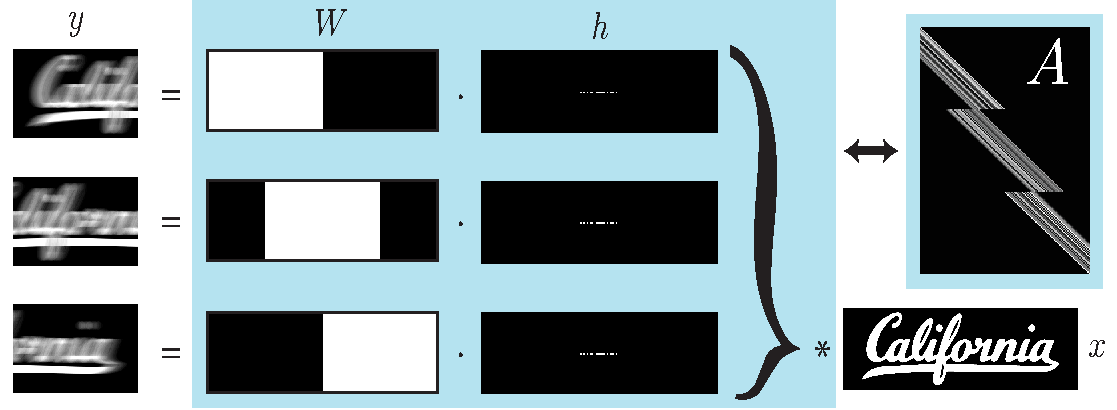
\includegraphics[width=\textwidth]{figures/fig_highthroughput_forward_model.pdf}
  \caption{\label{fig:forward_model}Multi-frame forward model. Here $[*]$ represents 2D convolution and $[\cdot]$ represents the element-wise product.}
\end{figure}

\subsection{Motion Blur Forward Models}
With knowledge of both sample trajectory and illumination sequence, the physical process of capturing a single measurement of a sample illuminated by a sequence of pulses while in motion can be mathematically described as a convolution:

\begin{equation}
\label{eq:single_forward}
\image = \kernel * \object + \noise,
\end{equation}

\noindent where $\image$ is the blurred measurement, $\object$ is the static object to be recovered, $\noise$ represents additive noise, $*$ represents 2D convolution, and $\kernel$ represents the blur kernel, the mapping of the temporal illumination intensity to positions in the imaging coordinate system using kinematic motion equations. With appropriate padding, this convolution can be computed efficiently using the Fourier Transform, and can be similarly inverted using FFT-based deconvolution.

To use coded illumination for large FOV imaging, we propose an extension of the single-frame forward model to the multi-frame case.
Mathematically, we model the serial acquisition of motion-blurred frames as the vertical concatenation of many single-frame forward models, which are individually convolutional (Fig.~\ref{fig:forward_model}).
In our model, each captured image has an associated blur operator $\B_j$ defined by each blur kernel $\h_j$ such that $\h_j * \x = \B_j \x$.
Additionally, we prepend each convolutional sub-unit with a crop operator $\W_j$, which selects an area of the object based on the field-of-view of the camera. Together, these operators encode both spatial coverage and the local blurring of each measurement, and are concatenated to form the complete multi-frame forward operator:

\begin{equation}
\label{eq:multiframe_forward}
\begin{bmatrix}\y_1\\ \vdots \\ \y_n \end{bmatrix} = \begin{bmatrix}\W_1\B_1 \\ \vdots \\ \W_n \B_n \end{bmatrix} \x + \noise = \A\x + \noise\:
\end{equation}

This forward operator $\A$ is no longer generally convolutional, taking the form of a spatially variant convolution based on the coverage of each individual $\W_j$. A one-dimensional illustration of the multi-frame smear matrix $\A$ is displayed in Fig.~\ref{fig:forward_model}.
With the addition of appropriate windowing logic, the forward operation and its adjoint can be computed efficiently for use in iterative reconstruction.

\begin{figure*}
  \centering
    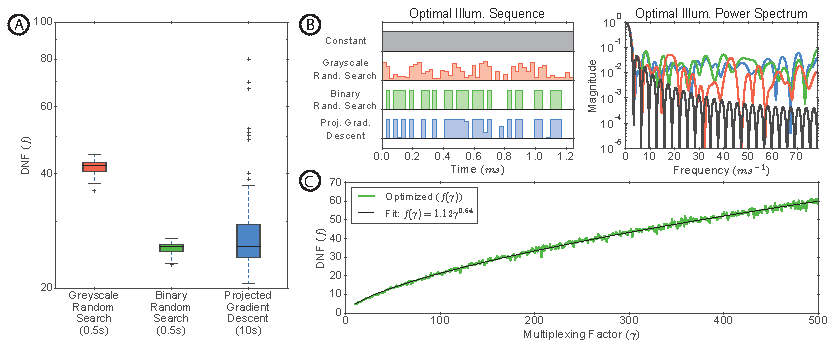
\includegraphics[width=\textwidth]{fig_highthroughput_illumination_optimization.pdf}

  \caption{ \label{fig:illum_optimization} A.) Resulting DNF values for illumination patterns generated by different optimization methods show that random search over binary patterns is of comparable effectiveness to the projected gradient descent method. B.) Example illumination sequences show differing power spectra between constant illumination and patterns generated by random search over greyscale, random search over binary, and projected gradient descent. C.) Optimized DNF (binary random search method) is plotted over different values of $\gamma$. A power law fit of $f(\gamma) = 1.12 \gamma^{0.641}$ has standard error of $1.075$.}
\end{figure*}

\subsection{Reconstruction Algorithm}\label{sec:recon}
To invert our forward model (Eq.~\ref{eq:multiframe_forward}), we employ Nesterov accelerated gradient descent~\cite{nesterov} algorithm to minimize the distance between our measurements $\y$ and estimated object $\widehat \x$ passed through forward model $\A$ in the $\ell_2$ metric. For the purposes of this work, we seek to minimize an unregularized cost function, $O(\x) = \frac{1}{2}\|\A\x - \y\|_2^2$ using the following update equation at each $k^{th}$ iteration:

\begin{equation}
    \label{eq:reconstruction}
    \x^{k+1} = \x^k - \alpha^k \A^\top (\A\x - \y)\:
\end{equation}
Here $\alpha^k$ is a scalar which is set each iteration by the Nesterov update equation.

In all reconstructions we performed 30 iterations of Eq.~\ref{eq:reconstruction}, which we found was a favorable balance of reconstruction quality and reconstruction time. While adding a regularization term such to enforce signal priors could improve reconstruction quality (and was previously analyzed in the context of motion deblurring~\cite{mitra:2014}), we chose not to incorporate regularization to provide a more fair and straightforward comparison between the proposed coded illumination acquisition and conventional strobed and stop-and-stare acquisitions. It should be noted that running our algorithm for a pre-defined number of iterations may provide some regularization from early-stopping~\cite{hagiwara2000regularization}.

Reconstructions were performed in Python using the Arrayfire GPU computation library~\cite{Yalamanchili2015}.
Due to the structure of our scans (Figure~\ref{fig:system}A), the reconstruction algorithm is highly parallelizable -- we separate our reconstruction into strips along the major translation axis to perform 1D convolutions, and stitch these strips together after computation.
Using this parallelization, we are able to reconstruct an approximately 1 gigapixel FOV in approximately 2 minutes. Further details of the reconstruction implementation are discussion in Section~\ref{sec:results}.

\subsection{Reconstruction SNR}\label{sec:methods_snr}

To minimize the error between the reconstructed $\widehat \x$ and the true object $\x$, the blur kernels and scanning pattern should be chosen such that the noise is minimally amplified by the inversion process. This amplification is controlled by the singular values of the forward model $\A$.

In the case of single-frame blur, the singular values are controlled by the length and coding of the blur kernel $\h$.
While early works~\cite{raskar2006coded, Ma:15} used a non-linear optimization routine (i.e. the \texttt{fmincon} function in MATLAB (Mathworks)) to minimize the condition number of $\A$, more recent work proposed maximizing the reconstruction signal-to-noise ratio directly, using camera noise parameters, source brightness, and the well-posedness of the deconvolution~\cite{agrawal2009optimal, cossairt2013does}.

We extend this work to the multiframe setting.
In our analysis, we adopt the convention of imaging SNR, which is the ratio of the mean signal to the signal variance (due to photon shot noise, camera readout noise, fixed pattern noise, and other camera-dependent factors). Under a simplified model, the noise variance will be the addition in quadrature of the camera read noise variance $\sigma^2_{r}$ plus a signal dependent term $\bar{s}$:

\begin{equation}
    \label{eq:snr}
    SNR = \frac{\bar{s}}{\sqrt{\bar{s} + \sigma^2_{r}}}\;
\end{equation}

Here, we ignore exposure-dependent noise parameters such as dark current and fixed-pattern noise, since these are usually small for short exposure times relative to read noise $\sigma^2$. Note that the denominator of Eq.~\ref{eq:snr} is equivalent to the standard deviation of $\noise$ in Eq.~\ref{eq:single_forward}. This definition is valid for both strobed illumination and stop-and-stare acquisitions. For an acquisition performed using coded illumination, it is necessary to consider the noise amplification that results from inverting the forward model. As defined in previous work~\cite{agrawal2009optimal}, this amplification is controlled by the deconvolution noise factor (DNF), which for single-frame blurring is defined as:

\begin{equation} \label{eq:DNF}
f = \sqrt{\frac{1}{m} \sum_{i=0}^m \frac{\max_i{|\tilde{\h}|_i^2}}{|\tilde{\h}|_i^2}}\:
\end{equation}
In Eq.~\ref{eq:DNF}, $m$ is the size of the blur kernel $\h$, and $\tilde{\h}$ represents the Fourier transform of $\h$. % Note that for a convolutional forward model, the magnitude of the Fourier coefficients of the kernel $\h$ ($|\tilde{\h}|$) are the singular values of the convolutional operator $\B$ which performs a convolution with $\h$.


\begin{figure*}
  \centering
    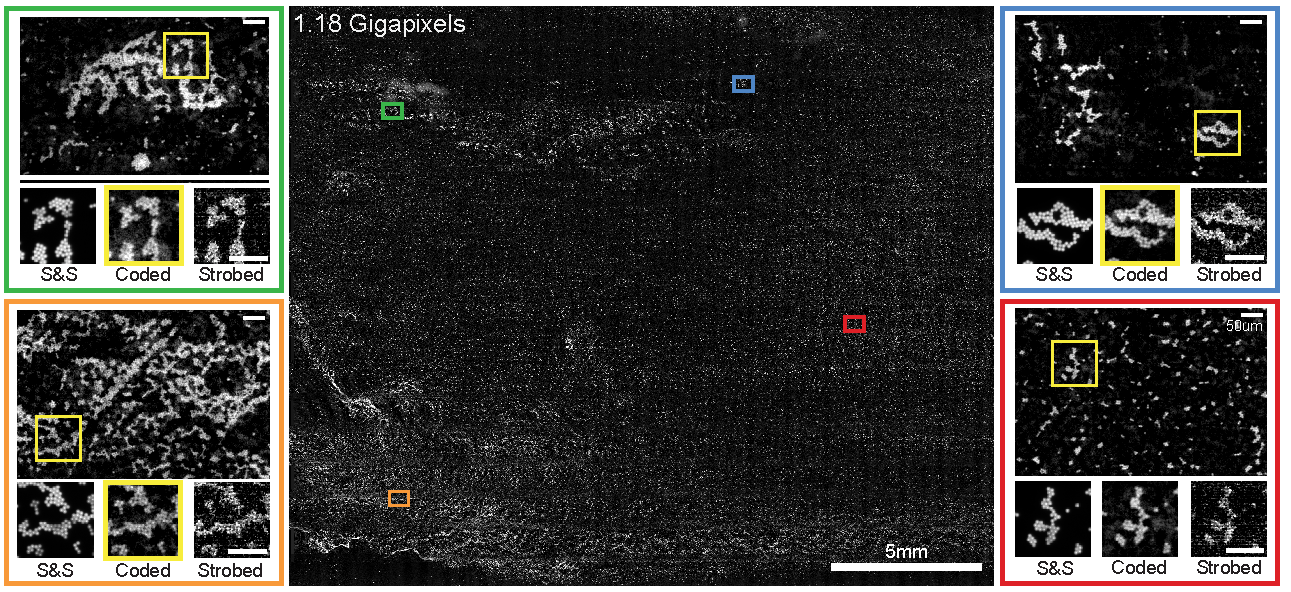
\includegraphics[width=1.0\textwidth]{figures/fig_highthroughput_full_field.pdf}

  \caption{(1.18 gigapixel, 23mm $\times$ 20mm full-field reconstruction of 4.7$\mu m$ fluorescent microspheres. Inset scale bars are 50$\mu m$. While coded reconstructions have lower SNR than stop-and-stare (S\&S) measurements, measurements acquired using coded illumination (Coded) were more than 5.5$\times$ faster while maintaining enough signal to distinguish individual microspheres compared to strobed illumination (Strobed)}

\end{figure*}

To write an expression for the singe-frame SNR under coded illumination, we first define a multiplexing factor $\gamma=\sum_{i} h_i$, the total amount of illumination imparted during exposure. If $\h$ is constrained to be binary, $\gamma$ will be equal to the number of pulses in $\h$. Eq.~\ref{eq:snr} can the be modified using both $f$ and $\gamma$:

\begin{equation}
    \label{eq:snr_coded}
    SNR  = \frac{\gamma\bar{s}_0}{f\sqrt{\gamma\bar{s}_0 + \sigma^2_{r}}}\:
\end{equation}
In Eq.~\ref{eq:snr_coded}, $\bar{s}_0$ is the mean signal imparted by a single illumination pulse. We include the complete derivation of~\eqref{eq:snr_coded} in Appendix~\ref{sec:snr_derivation} for completeness.

The derivation of this quantity relies on the convolutional nature of single-frame motion blur.
However, the multi-frame forward operator $\A$ has the form of a spatially variant convolution matrix. As shown in Fig.~\ref{fig:forward_model},
each column of this matrix defines a localized convolutional kernel; near the horizontal boundaries between the different frames, the vertical combinations of kernels are non-trivial.
While methods for analyzing spatially variant convolution matrices exist~\cite{chan2011bounds}, we focus our analysis on a practical simplifying assumption: blur path and illumination patterns are fixed to be the same across all frames, i.e. $\h_j=\h$ for all $j$.

In this special case, the resulting SNR of the proposed multi-frame model is governed by both the power spectrum of the blur kernel and the spatial coverage of the crop operators. We define $c_i$ to be the \textit{coverage} at pixel $i$, i.e. the number of times pixel $i$ is included in the windows $\{\W_1,...,\W_n\}$.
The SNR for a multi-frame acquisition with coded illumination is bounded as
\begin{align*}
    SNR  \geq \sqrt{
    \min_{i} c_i}  \cdot \frac{ \gamma\bar{s}_0}{f\cdot \sqrt{\gamma\bar{s}_0 + \sigma^2_{r}}}\:
\end{align*}

Thus, the SNR improves by at least a factor of square root the minimum coverage compared with the single-frame coded illumination case in~\eqref{eq:snr_coded}. The derivation is included in Appendix~\ref{sec:multiframe_app}.

Notably, this bound decouples the spatial coverage from the spectral quality of the blur, allowing for blur kernel optimization independent of the multi-frame aspect. A good motion path ensures even spatial coverage through $c_i$ while a good illumination sequence ensures spectral coverage through traditional single-frame methods. In what follows, we focus system design on the maximization of this decoupled lower bound.

The decision to use the same blur kernel in every frame has several practical implications as well: the micro-controller memory would be saturated when storing more than one thousand kernels and post-processing registration is much easier since all measurements have been distorted by the same blurring operator. Additionally, the fact that this reduction requires the motion to be along single motion axis is not limiting, since in practice horizontal strips are reconstructed independently to accommodate computer memory.

\subsection{Illumination Optimization}\label{sec:illum_opt}
Previous work~\cite{raskar2006coded, agrawal2009optimal} showed that reconstructions performed using constant (non-coded) illumination will have very poor quality (in terms of SNR) compared to using optimized pulse sequences or a short, single pulse. Here, we explore several approaches for generating illumination pulse sequences which maximize the reconstruction SNR (Eq.~\ref{eq:snr_coded}). We first consider the problem of minimizing the DNF ($f$) with respect to $\h$:
\begin{align}
    \begin{split}
        \label{eq:illum_opt_single}
        f(\gamma) := \min_{\h}&~~ f \\
          s.t. &~~0 \leq h_i \leq 1 \; \forall \; i, \quad
          \sum_{i} h_i = \gamma \:,
    \end{split}
\end{align}

\noindent where inequality constraint on $\h$ represents the finite optical throughput of the system.
This optimization problem is non-convex, and it resembles those used in previous work~\cite{raskar2006coded,agrawal2009optimal,Ma:15} (Our multiplexing factor $\gamma$ is related to the kernel length $N$ and throughput coefficient $\beta$ in previous work by $\gamma = N\beta$). This definition enables a divide-and-conquer approach to maximizing the SNR: after solving Eq.~\ref{eq:illum_opt_single} for each multiplexing factor, it is possible to find the one which optimizes~\eqref{eq:snr_coded} in the context of camera noise parameters.

To simplify the optimization task, the positions encoded in $\h$ may be restricted a priori, e.g. to a centered horizontal line with length as in Fig.~\ref{fig:forward_model}. In the following, we positions to a straight line with length $N=2\gamma$. This provides a sufficiently large sample space for kernel optimization, and is supported as optimal by analysis in~\cite{agrawal2009optimal}.

We consider several methods for solving the DNF optimization in Eq.~\ref{eq:illum_opt_single}: random search over greyscale kernels, random search over binary kernels, and a projected gradient descent (PGD) approach. Our random search approach is simple: a fixed number of binary candidate kernels are randomly generated, and the one with the lowest DNF is chosen. Similarly, grayscale random candidates were generated by sampling uniform random variables, while the binary were generated by sampling indices without replacement. In our PGD approach, the kernel optimization problem (Eq.~\ref{eq:illum_opt_single} is reformulated as the minimization of a smooth objective $g(\h)$ subject to convex constraints $\mathcal{S}$.

Starting from an initial $\h_0$, the update rule includes a gradient step followed by a projection:
\begin{align*}
    \tilde \h^{k+1} &= \mathrm{Proj}_{\mathcal{S}}(\h^k - \alpha^k \nabla g(\h))\:.
\end{align*}
Details of the reformulation and optimization approach are presented in Appendix~\ref{sec:optimization_app}.

The box plots in Fig.~\ref{fig:illum_optimization}A show the distribution of optimization results for 100 trials of each approach, where the random search methods sample 1000 candidates and PGD runs with step-size determined by backtracking line search until convergence from a random binary initialization. Example illumination sequences from each method and their corresponding power spectra are displayed in Fig.~\ref{fig:illum_optimization}B.

Though the kernels with the lowest DNF were generated through PGD, binary random search results in comparable DNF values and is up to $20\times$ faster than PGD. Further, we note that a random binary search resulted in significantly lower DNF calculations than grayscale random search. A binary restriction also achieves fast illumination updates, since grayscale illumination (as in~\cite{Ma:15}) would require a pulse-width-modulation (PWM) cycle spread across multiple clock cycles.

Plotting $f(\gamma)$ generated through binary random search in Fig.~\ref{fig:illum_optimization}C reveals a concave curve. Fitting this to a power-law function We find a closed-form approximation for the DNF as a power law with $f(\gamma)=1.12\gamma^{0.64}$. This analytic relationship allows for a direct optimization of SNR: substituting any $f(\gamma) \propto \gamma^p$ into Eq.~\ref{eq:snr_coded} and differentiating with respect to $\gamma$, we can determine the approximately optimal multiplexing factor $\gamma^*$ as a function of mean strobed signal $\bar{s}_0$ and camera readout noise $\sigma_r^2$:

\begin{equation}
    \label{eq:optimal_gamma}
    \gamma^* = \frac{2-2p}{2p-1} \cdot \frac{\sigma_r^2}{\bar{s}_0}\:.
    % \frac{2.57143 \cdot \sigma_r^2}{\bar{s}_0}
\end{equation}

We note that for smaller $p$, i.e. slower DNF growth with $\gamma$, the optimal multiplexing factor will be larger.
The experimental $p=0.64$ accurately reflects the practical relationship, given that we experience limitations from imperfect optimization methods. Part of the observed relationship may come from the the increasing difficultly of optimization as the decision space grows with $\gamma$. However, we show in Appendix~\ref{sec:dnf_limit} the lower bound $f(\gamma)\geq \gamma^{0.5}$ regardless of optimization method or illumination sequence.

The expression for optimal $\gamma^*$ also solidifies the intuition that a higher $\gamma$ should be used for systems with high noise in order to increase detection SNR, while a lower multiplexing is appropriate for less noisy systems. This result is in agreement with~\cite{agrawal2009optimal}, in which it was demonstrated that the choice of multiplexing factor depends on the relative magnitude of the acquisition noise.

\subsection{System Hardware and Software} \label{Sec:hardware}
Our system is built around a inverted microscope (TE300 Nikon) using a lateral motion stage (Prior, H117). Images were acquired using a SCMOS camera (PCO.edge 5.5, PCO) through hardware triggering, and illumination was provided by a high-power LED (M470L3, Thorlabs) which was controlled by a micro-controller (Teensy 3.2, PJRC). Brightfield measurements were illuminated using one of two sources: a custom LED illuminator with 40 blue-phosphor LEDs (VAOL-3LWY4, VCC), or a single, high-power LED source (Thorlabs M470L3), both modulated using a simple single-transistor circuit through the same micro-controller. The first illuminator was designed to have a broad spectrum for brightield imaging, while the second was intended for fluorescence imaging, having a narrow spectral bandwidth. For this project, we found it was necessary to adopt very simple LED circuitry to avoid electronic speed limitations associated with dimming (PWM) and serial control of LED driver chips. A schematic and layout of our system is shown in Fig.~\ref{fig:system}A and a photograph in Fig.~\ref{fig:system}C.

The micro-controller firmware used in this device was developed as part of a broader open-source LED array firmware project~\cite{illuminate}. Images were captured through the python bindings of the Micro-Manager software~\cite{micromanager}, which were controlled through a Jupyter notebook~\cite{Kluyver:2016aa}, enabling fast prototyping of both acquisition and reconstruction pipelines in the same application. With the exception of our custom illumination device, everything in our optical system is commercially available in combinations commonly available at many imaging centers. Therefore, our method is amenable to most traditional optical setups, and can be implemented cheaply through the simple addition of our temporally coded light source and open-source software tools.

All acquisitions in this work were performed using a 10$\times$, 0.25NA objective, which had a depth of field of approximately 8.5 $\mu m$. Because this depth-of-field was relatively large compared to our sample, we were able to level the sample manually prior to acquisition using adjustment screws present on the motion stage to ensure the sample remained in focus across an approximately 20$mm$ movement range. For larger areas or shallower DOF, we anticipate a more sophisticated leveling technique will be necessary, such as active autofocus~\cite{nikonperfect, zeissdefinite}. In practice, the focal adjustment process required only a few minutes for our 10$\times$ objective, and was stable between samples (requiring infrequent adjustment).

\subsection{Results}\label{sec:results}
To demonstrate the performance benefit of our system, we performed a 1.18 gigapixel reconstruction of a microscope slide plated with 4.7$\mu m$ polystyrene fluorescent beads (Thermo-Fisher) using the high-throughput coded illumination microscope shown in Fig.~\ref{fig:system}. Multiple images were captured at spatial offsets, enabling a reconstruction with extend field of view (FOV). Each scan pathways consisted of multiple 1D continuous scans while imaging structured in a raster-scanning pattern (Fig~\ref{fig:forward_model}{B}) to enable fast 2D scanning of the sample. For a complete comparison, we acquired stop-and-stare, strobed illumination, and coded illumination datasets serially, and performed image stitching and registration of the three datasets for a direct comparison of image quality. The total acquisition time for the coded reconstructions of this size was 31.6 seconds, while a comparable stop-and-stare acquisition required 210.9 seconds. The computation time for coded-illumination reconstructions was approximately 30 minutes on a Macbook Pro (Apple) with attached RX580 external GPU (Advanced Micro-Devices), or approximately 2 minutes when parallellized across 18 EC2 cloud computation p2.xlarge instances with Nvidia Titan GPUs (Amazon Web Services), excluding data transfer to and from our local machine.

\begin{figure}
\centering
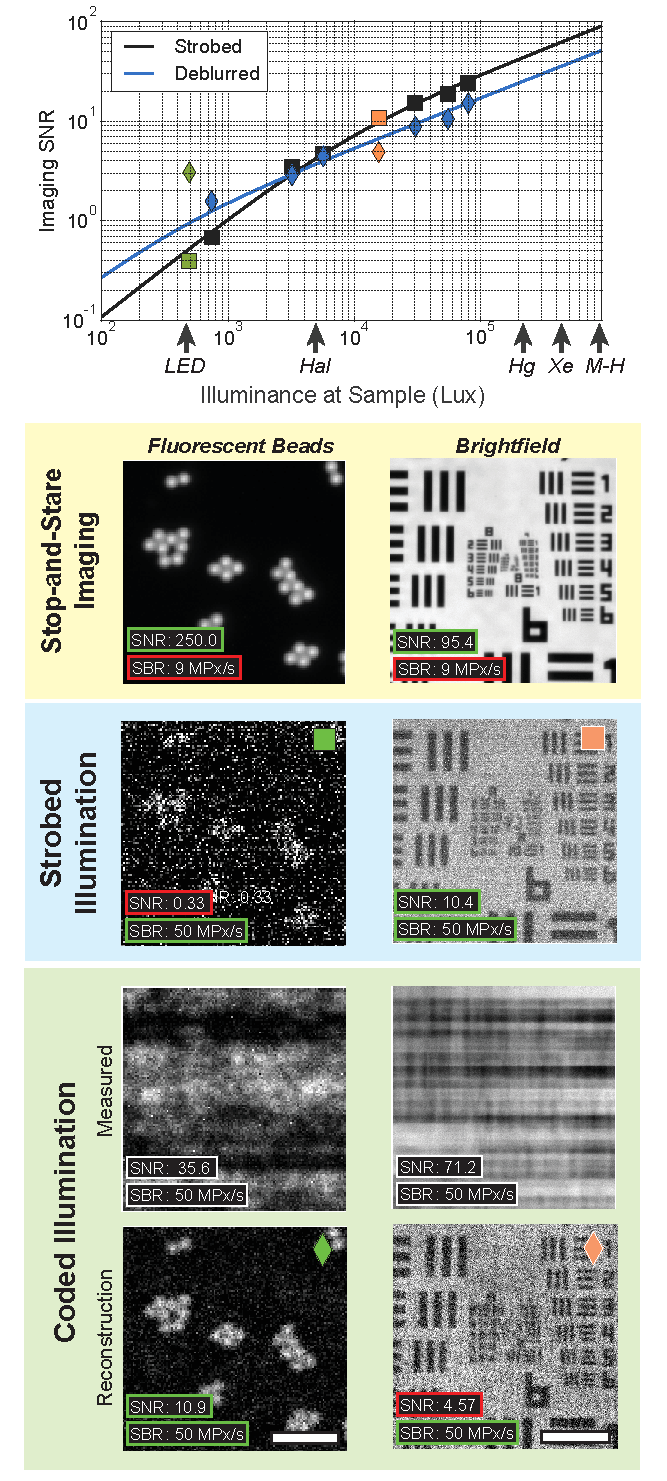
\includegraphics[width=0.48\textwidth]{figures/fig_highthroughput_snr_comparison.pdf}
  \caption{\label{fig:experimental_comparison}(Top) Experimental SNR values for a USAF 1951 resolution illuminated across a range of illumination values under strobed (square) and coded illumination (diamond). Solid lines illustrate predicted SNR based on known system parameters. Experimental SNR values are the average of 3 SNR measurements performed across the field. Green and orange data points represent inset data for fluorescent beads and resolution targets respectively. Characteristic illuminance values for LED sources, Halogen-Tungsten Lamps (Hal.), Mercury Lamps (Hg), Xenon Lamps (Xe), and Metal-Halide Lamps (M-H) are shown for reference. (Bottom) Selection of measurements used to generate the above plot. Scale bar is 25 $\mu m$.}

\end{figure}

To provide a complete comparison of our coded illumination method with existing high-throughput imaging techniques, we sought to quantify the expected SNR for each method based on relevant system parameters such as source illuminance, camera noise parameters, and desired acquisition frame-rate. In conventional high-throughput imaging it is well-understood that stop-and-stare strategy will provide higher SNR than imaging using strobed illumination, but is only feasible for low-frame rates due to mechanical limitations of the motion stage. Our method (coded illumination) can be thought of as an improvement of strobed illumination for acquisitions with a high-frame rate requirement; however, coded illumination will nearly always be sub-optimal compared to stop-and-stare illumination at low-frame rates due to extended exposure times without additional deconvolution noise. Therefore, at high frame-rates we restrict our comparison to strobed illumination and coded illumination. Later, we perform a comprehensive analysis of these trade-offs; Fig.~\ref{fig:component_analysis}A provides a visual representation of where stop-and-stare is possible in terms of mechanical parameters of the motion stage.

Using the experimental setup described in Fig~\ref{fig:system} we performed experimental comparison of acquisitions performed under brightfield and fluorescence configurations while sweeping the output power of the LED source. In each case, we measured the illuminance at the camera plane using an optical power meter (Thorlabs). For each image and reconstruction we computed the average imaging SNR across three different regions of interest to produce an experimental estimate of the overall imaging SNR of the scene. To ensure a fair comparison, we performed no prepossessing on the data except for subtracting a known, constant offset from each measurement which was characterized before acquisitions were performed and verified with the camera datasheet. Reconstructions of measurements made using coded illumination were performed using the reconstruction algorithm described in Section 2\ref{sec:recon}.

Fig.~\ref{fig:experimental_comparison} shows that coded illumination can provide up to $10\times$ higher SNR in low-illumination situations, which are most relevant for fluorescence microscopy (illuminance < 1000 lux). For brightfield microscopy, strobed illumination provides a higher SNR without additional computational complexity associated with our coded illumination method. The solid lines in Fig.~\ref{fig:experimental_comparison} are theoretical predictions of reconstruction SNR for each method based on our system parameters, which are generally in agreement with our experimental data. The methods for computing these curves are described in section~\ref{sec:highthroughput_component_analysis}.

\section{SNR Analysis of High-Throughput Imaging Systems}\label{sec:highthroughput_component_analysis}

\begin{figure*}
  \centering
    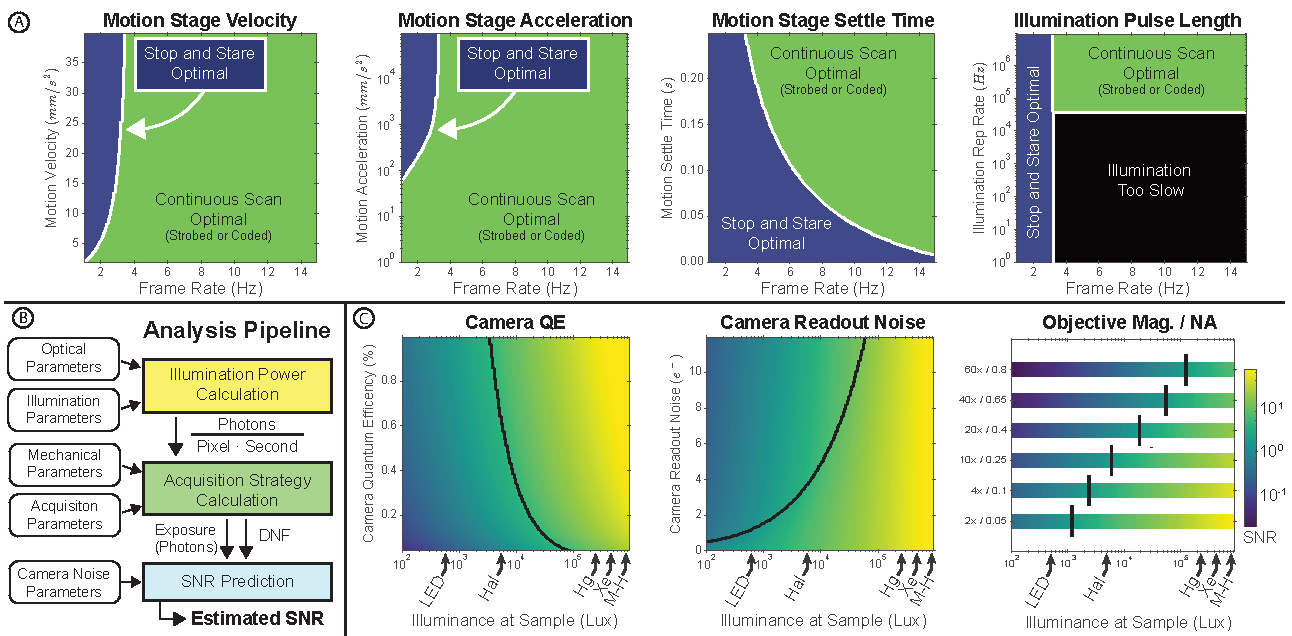
\includegraphics[width=1.0\textwidth]{figures/fig_highthroughput_limiting_analysis.pdf}
      \caption{\label{fig:component_analysis} Limiting Analysis of Imaging System. A.) Analysis pipeline for predicting SNR from system parameters, including illumination power, mechanical parameters of the motion stage, and camera noise parameters. B.) The stop-and-stare acquisition strategy is only possible for some configurations of mechanical system parameters and frame rates. C.) Different combinations of optical system parameters and system illuminance determine the best possible SNR and whether strobed or coded illumination is preferable. Characteristic illuminance values for LED sources, Halogen-Tungsten Lamps (Hal), Mercury Lamps (Hg), Xenon Lamp (Xe), and Metal-Halide Lamps (M-H) are shown for reference. }
\end{figure*}

In the previous section, we showed that choice to use strobed or coded illumination depends heavily on the illumination power of the source; however, other system parameters may also affect this trade-off. In this section, we extend this to include other parameters such as camera noise and motion velocity, and include an analysis of when stop-and-stare should be used as opposed to continuous-scan methods (strobed illumination and coded illumination). As a first step, we derive the expected photons per pixel, per second ($J$) we expect to measure in a transmission microscope, incorporating system magnification ($M$), numerical aperture ($NA$), camera pixel size ($\Delta$), mean wavelength ($\bar{\lambda}$, and the photometric look-up table $K(\bar{\lambda})$:

\begin{equation}
\label{eq:photonflux}
J = K(\bar{\lambda}) \bar{\lambda}\hbar c \cdot I_{lux} * (NA)^2 * (\frac{\Delta}{M})^2
\end{equation}

Here, $\hbar$ is Planck's constant, $c$ is the speed of light, $I_{lux}$ is the source illuminance in lux, and $J$ is the photon flux per pixel-second. Given $J$, the mean signal $\bar{s}$ is a function of the illumination time $t_{illum}$ and the camera quantum efficiency $Q$:

\begin{equation}
\label{eq:illuminance_to_signal}
    \bar{s} = J Q t_{illum}
\end{equation}

Substituting Eq.~\ref{eq:illuminance_to_signal} into Eq.~\ref{eq:snr_coded}, we can define the expected SNR as a function of these parameters as well as the blur kernel $h$ and camera readout noise $\sigma_r$:

\begin{equation}
\label{eq:photonflux_snr}
SNR = \frac{J Q t_{illum}}{f \sqrt{J Q t_{illum} + \sigma_r^2}}
\end{equation}
Eq.~\ref{eq:photonflux_snr} is used in the analysis of Fig.~\ref{fig:experimental_comparison} and Fig.~\ref{fig:component_analysis}.

The parameters $t_{illum}$ and $f$ are functions which change based on acquisition strategy.
For stop-and-stare and strobed acquisitions, we set $f = 1$, since no deconvolution is being performed, while for coded acquisitions $f$ depends on the parameter $\gamma$ as derived in Section 2\ref{sec:illum_opt}.
Similarly, $t_{illum}$ is set based on acquisition strategy and motion stage parameters. For stop-and-stare illumination, $t_{illum}$ is proportional to the residual time after stage movement, including stage acceleration ($v_{stage}$), the field of view of a single frame along the blur axis ($FOV$), mechanical settle time ($t_{stage}$), and desired acquisition frame rate $r_{frame}$:

\begin{equation}
\label{eq:sns_illum}
t_{illum} = \frac{1}{r_{frame}} - 2\frac{v_{stage}}{a_{stage}} - \frac{FOV - 0.5 * \frac{v_{stage}^2}{a_{stage}}}{v_{stage}}\:.
\end{equation}

For strobed and coded illumination, the minimum pulse duration $t_{illum}$ is set by the overlap fraction ($O$) between frames, the number of pixels along the blur direction, $N_{px}$, and the multiplexing by $\gamma$ (with strobed encoded by $\gamma=1$):

\begin{equation}
\label{eq:strobed_coded_illum}
t_{illum} = \frac{\gamma}{r_{frame}(1 - O) N_{px}}\:.
\end{equation}
In Eq.~\ref{eq:strobed_coded_illum}, we implicitly calculate the velocity as the fastest speed where two frames may overlap with $O$ within a time set by $r_{frame}$.

Derivations for the above relationships are provided in Appendix~\ref{sec:app_throughput}. With these theoretical solutions for $t_{illum}$, we are able to derive closed-form solutions for expected SNR as a function of acquisition rate with knowledge of our system parameters (Listed in Appendix~\ref{sec:sys_param}), using the pipeline shown in Fig.~\ref{fig:component_analysis}B.

Our system analysis is divided into two parts; When stop-and-stare is possible given a desired acquisition frame rate, it will always provide higher SNR than strobed or coded illumination due to high photon counts compared to strobed illumination and no deconvolution noise. Fig.~\ref{fig:component_analysis}A analyzes where stop-and-stare is both possible and optimal compared to a continuous acquisition technique as a function of frame rate. If acquisition frame rate is low or limited by other factors (such as sample stability), stop-and-stare will always be optimal in terms of SNR. If a high-frame rate is desired, however, a continuous acquisition strategy is optimal, so long as the illumination repetition rate of the source is fast enough to accommodate sample velocity.

Fig.~\ref{fig:component_analysis}C describes the optimal continuous imaging technique as a function of illuminance, imaging objectives, camera readout noise ($\sigma_r$, and camera quantum efficiency ($QE$). Generally speaking, higher illuminance values favor strobed illumination (being shot-noise limited), while lower illuminance values favor coded illumination (being read-noise limited). Conversely, as read noise ($\sigma_r$) increases or camera $QE$ decreases, coded illumination becomes more beneficial. Practically, a camera with high read-noise with a low $QE$ will favor coded illumination more strongly (at higher source illuminance) than a high-end camera (such as the PCO.edge 5.5 used in this study), where $\sigma_r \approx 3.7 e^-$ and $QE \approx 0.6$). In addition, objectives with a higher magnification and NA will generally favor coded illumination more strongly due to the decreasing $\frac{NA}{Mag}$ ratio, although this is not necessarily true for all NA/magnification combinations due to differing optical designs. It should be noted, however, that higher NA values will require more sophisticated autofocusing methods than those presented in this work. Example illuminance values for common microscope sources were calculated based on estimated source power at 550nm~\cite{illumpower}.

\section{Summary}
In this chapter, we have demonstrated a novel high-throughput imaging framework which employs multi-frame motion deblurring using coded illumination. Through both experiment and theoretical analysis we have shown the applicability of out method for fluorescence microscopy, and performed a comprehensive analysis of when our method makes sense in terms of source power and other system parameters. These results indicate that coded illumination provides up to $10\times$ higher SNR than conventional strobed illumination methods in low-light situations, making our method particularly well-suited for applications in drug-discovery and whole-slide imaging. Our analysis of optimal kernel selection indicates that efficient illumination sequences can be calculated quickly and cheaply using a simple random search, and our analysis of optimal pulse length provides an approximate relationship between the length of a pulse sequence and source illuminance. Further, our proposed multi-frame reconstruction algorithm produces good results using simple accelerated gradient descent with no regularization, and can be scaled to multiple cloud instances for fast data processing. Future work should address improvements such as regularization, more complicated motion pathways, self-calibration, and reconstructions using under-sampled data.